\chapter{Metodología}
\section{Alcance de la Investigación}

\section{Datos de entrada al modelo}
\subsection{Bases de datos utilizadas}
\subsubsection{Información Geográfica}
La información estática que sirve como condición de borde inferior al modelo debe extraerse de datos satelitales u otros similares con el objetivo que sea uniforme y confiable. Esta información debe ser siempre georeferenciada (protocolo GIS).

WRF utiliza una base de datos estática lo suficientemente amplia como para poder satisfacer un uso normal del modelo, sin embargo, si se desea utilizar WRF en condiciones extremas, es decir, a escalas lo suficientemente pequeñas como para que las bases de datos no satisfagan la resolución, es necesario actualizar algunas bases de datos. La información a actualizar debe ser:
\begin{itemize*}
	\item Altura del Terreno: Para una obtención precisa de los niveles $\eta$ en cada punto del dominio y por lo tanto una correcta representación del terreno complejo que va a ser el principal motivador de la turbulencia.
	\item Uso de Suelo: Posee la información acerca del \% de vegetación, coeficiente térmico superficial y, lo más importante, el coeficiente de rugosidad ($z_0$), que es el parámetro a utilizar para estimar los flujos superficiales.
\end{itemize*}
Las bases de datos a utilizar en las simulaciones serán:
\begin{itemize*}
	\item GMTED2010: Dataset por defecto del WRF para la altura del terreno. Obtenida el año 2010 por la USGS y la NGA con una resolución de 30'.
	\item ASTER: Es el único instrumento de alta resolución de la NASA ubicado en la plataforma Terra. Esta base de datos se hizo pública el año 2011 y entrega información de la altura del terreno con una resolución de 1' ($\approx 30$ [m]).
	\item MODIS: Información obtenida por lo satélites de la nasa. Entregan información en 20 categorías a una resolución de 15' de arco.
	\item Corine: Obtenida el año 2012 (proyecto CLC12) a través de imágenes satelitales con 100m de resolución para toda Europa. Posee 44 categorías y es la base de datos de uso de suelo abierta de más alta resolución existente hasta ahora. Para este trabajo se usa la versión 18.5 modificada del año 2016.
	\item Bolund: Los autores del experimento de Bolund entregan bases de datos de la orografía del terreno y el coeficiente de rugosidad para este con una resolución de 25 [cm]
\end{itemize*}
\subsubsection{Incorporación a WRF}
La manera en la que los datos descritos anteriormente son entregados, muchas veces no están en el formato en el que el preprocesador del modelo WRF (WPS) puede asimilarlo. Sin embargo, debido a los estándar exigidos para información georeferenciada, es posible manipularla de tal manera que puedan incorporarse al modelo. A continuación se describen algunos trabajos que debieron hacerse con las bases de datos.
\begin{enumerate*}
	\item ASTER: Cambio de formato de GeoTiff a binario.
	\item Bolund Oro.: La información entregada por el experimento Bolund viene dada en un datúm UTM Z32, por lo cuál se debe transformar a WSG84, además, debido a la lectura de la información, los autores trasladaron las coordenadas, por lo cual hubo que invertir esta traslación. Se debió transformar la altura del agua entregada (los autores por motivos de interpolación de mareas declaran un $z=0.75$ para agua) a un nivel de $z=0$, para un correcto uso del modelo. 
	\item Corine: Se debió transformar su datúm nativo de ETRS89 a WSG84 Debido a que la clasificación de suelo por Corine no está implementada en WRF, se debe hacer un remapeo de los índices al formato USGS. Este procedimiento está descrito en Pineta et. al. (2004). Por otra parte, la resolución de los datos CLC12 son bastante gruesos en comparación con los entregados por ASTER 1s, luego el WPS presentó algunos errores en reconocer las masas de tierra y para solucionar esto se procedió a hacer una afinación manual de los datos CLC12 en las zonas relevantes para la simulación. Esta afinación puede verse en las figuras anexas a este informe.
	\item Bolund LU: Los autores del experimento entregan información acerca del $z_0$ en el dominio de Bolund y en el mismo formato en el que entregan la orografía, por lo tanto se debieron hacer las mismas trasformaciones detalladas anteriormente y luego hacer calzar la información entregada con un índice de tipo de suelo y que además fuera consistente con las bases de datos de uso de suelo usadas en los dominios mas grandes.
\end{enumerate*}
\subsubsection{Condiciones Iniciales y de Borde del Modelo}
Para inicializar el modelo y para proveer de información en los contornos cada 6 horas, se utilizan los datos de los análisis operacionales provenientes del modelo global GFS con resolución de $0.5^\circ$ ($\approx 55.6$ [km])

Por otra parte, como el dominio mas grande a simular cae dentro de lo que es una simulación de mesoescala y tomando en consideración las proyecciones debido a la curvatura de la tierra para esta zona en particular, se decide fijar la condición de borde superior para la coordenada vertical de presión a $p_{dht} = 5000$ [kPa] siguiendo la recomendación del manual del programa.

La condición de borde inferior queda determinada por la información obtenida en los datos de uso de suelo para cada punto de la malla.
\section{Preproceso de la Asimilación de Datos}

\section{Posproceso de los datos}
\subsection{Interpolación de alturas}
ley logaritmica.
\subsection{Cálculo de Errores}
Considerando que el resultado final de las simulaciones realizadas es un archivo de texto con la serie de tiempo para los valores de $u,v$ y $w$ para cada punto de interés en el dominio, es necesario definir una estimación del error entre la simulación realizada y la serie de tiempo medida en el mástil.

Se decide utilizar dos indicadores para llevar a cabo esta tarea: el MAE y el RMSE.

El MAE (\emph{Mean Absolute Error}) entre dos variables continuas se calcula de la siguiente forma:

\be 
MAE = \frac{1}{n}\sum_{i=1}^n |y_i-x_i|
\ee

Es un promedio del valor absoluto de los errores.

Si graficáramos la correspondencia de los datos en un gráfico de $x$ vs $y$, el MAE correspondería al valor medio de la distancia horizontal entre cada punto y la línea $x=y$.

El RMSE (\emph{Root Mean Squared Error}) por otro lado se calcula como:

\be 
RMSE = \sqrt{\frac{1}{n}\sum_{i=1}^n (y_i-x_i)^2}
\ee

Y corresponde a la raíz de los momentos muestrales de segundo orden de la diferencia entre los valores a comparar, en otras palabras, es un análogo al MAE pero pondera con mayor importancia los errores mas grandes. Es un promedio de los errores al cuadrado.
\section{Caso de Validación: Terreno Plano Høvsøre}
\subsection{Aspectos generales de las simulaciones}

\begin{table}[h!]
	\caption{Dominio numerico espacial y temporal para simulación del caso Høvsøre.}\label{tab:exp}
	\centering\footnotesize
	\begin{tabular}{lcc}
		\toprule
		Parámetro & Selección \\
		\midrule
		Fecha	 	 & 2010-09-08   \\
		Hora Inicio	 	 & 06:00:00   \\
		Hora Término	 		 & 20:00:00  \\
		Puntos Malla Vert.	 	 & 47   \\
		$P_{top}$ 	& 5000 kPa\\
		\# Dominios	& 7   \\
		Lat. Centro	& 56.447984   \\
		Lon. Centro	& 8.151570   \\
		\bottomrule
	\end{tabular}
\end{table}

\begin{table}[h!]
	\caption{Valores característicos de cada dominio.}\label{tab:param_fis}
	\centering\footnotesize
	\begin{tabular}{llllllll}
		\toprule
		Dominio 				& d01	&	d02	&	d03	&	d04	&	d05	&	d06 &	d07 \\
		\midrule
		$N_x$		& 107 & 107 & 107 &107&107&107&107  \\
		$N_y$	 		& 107 & 107 & 107 &107&107&107&107  \\
		$\Delta x = \Delta y$	[m]	 		& 30000 & 10000 & 3333.3 &1111.1&222.22&74.074&24.691  \\
		$\Delta t$	[s]	 		& 90 & 30 & 10 &3.333&0.666&0.222&0.074  \\
		Orografía		 	& GMTED2010 & GMTED2010 & GMTED2010 &ASTER&ASTER&ASTER&ASTER  \\
		Uso de Suelo					& USGS & USGS & USGS &CLC12&CLC12&CLC12&CLC12 \\
		\bottomrule
	\end{tabular}
\end{table}

\begin{table}[h!]
	\caption{Parametrizaciones físicas utilizadas en el modelo.}\label{tab:param_fis}
	\centering\footnotesize
	\begin{tabular}{llllllll}
		\toprule
		Dominio 				& d01	&	d02	&	d03	&	d04	&	d05	&	d06 &	d07 \\
		\midrule
		Micro-físicas		 	& WSM5 & WSM5 & WSM5 &WSM5&WSM5&WSM5&WSM5  \\
		Cúmulos			 		& Grell & Grell & -- & -- & -- & -- & -- \\ 
		Capa Superficial	 	& MM5 & MM5 & MM5 & MM5 & MM5 & MM5 & MM5 \\
		PBL				 		& YSU & YSU & YSU & YSU & -- & -- & -- \\
		Modelo LES				 		& -- & -- & -- & -- & 1.5TKE & 1.5TKE & 1.5TKE \\
		Modelo de Suelo 		& Difus. & Difus. & Difus. & Difus. & Difus. & Difus. & Difus. \\
		Rad. Onda Larga	& RRTM &RRTM&RRTM&RRTM&RRTM&RRTM&RRTM \\
		Rad. Onda Corta	& Dudhia &Dudhia&Dudhia&Dudhia&Dudhia&Dudhia&Dudhia \\
		\bottomrule
	\end{tabular}
\end{table}

\begin{figure}[H]
	\centering
	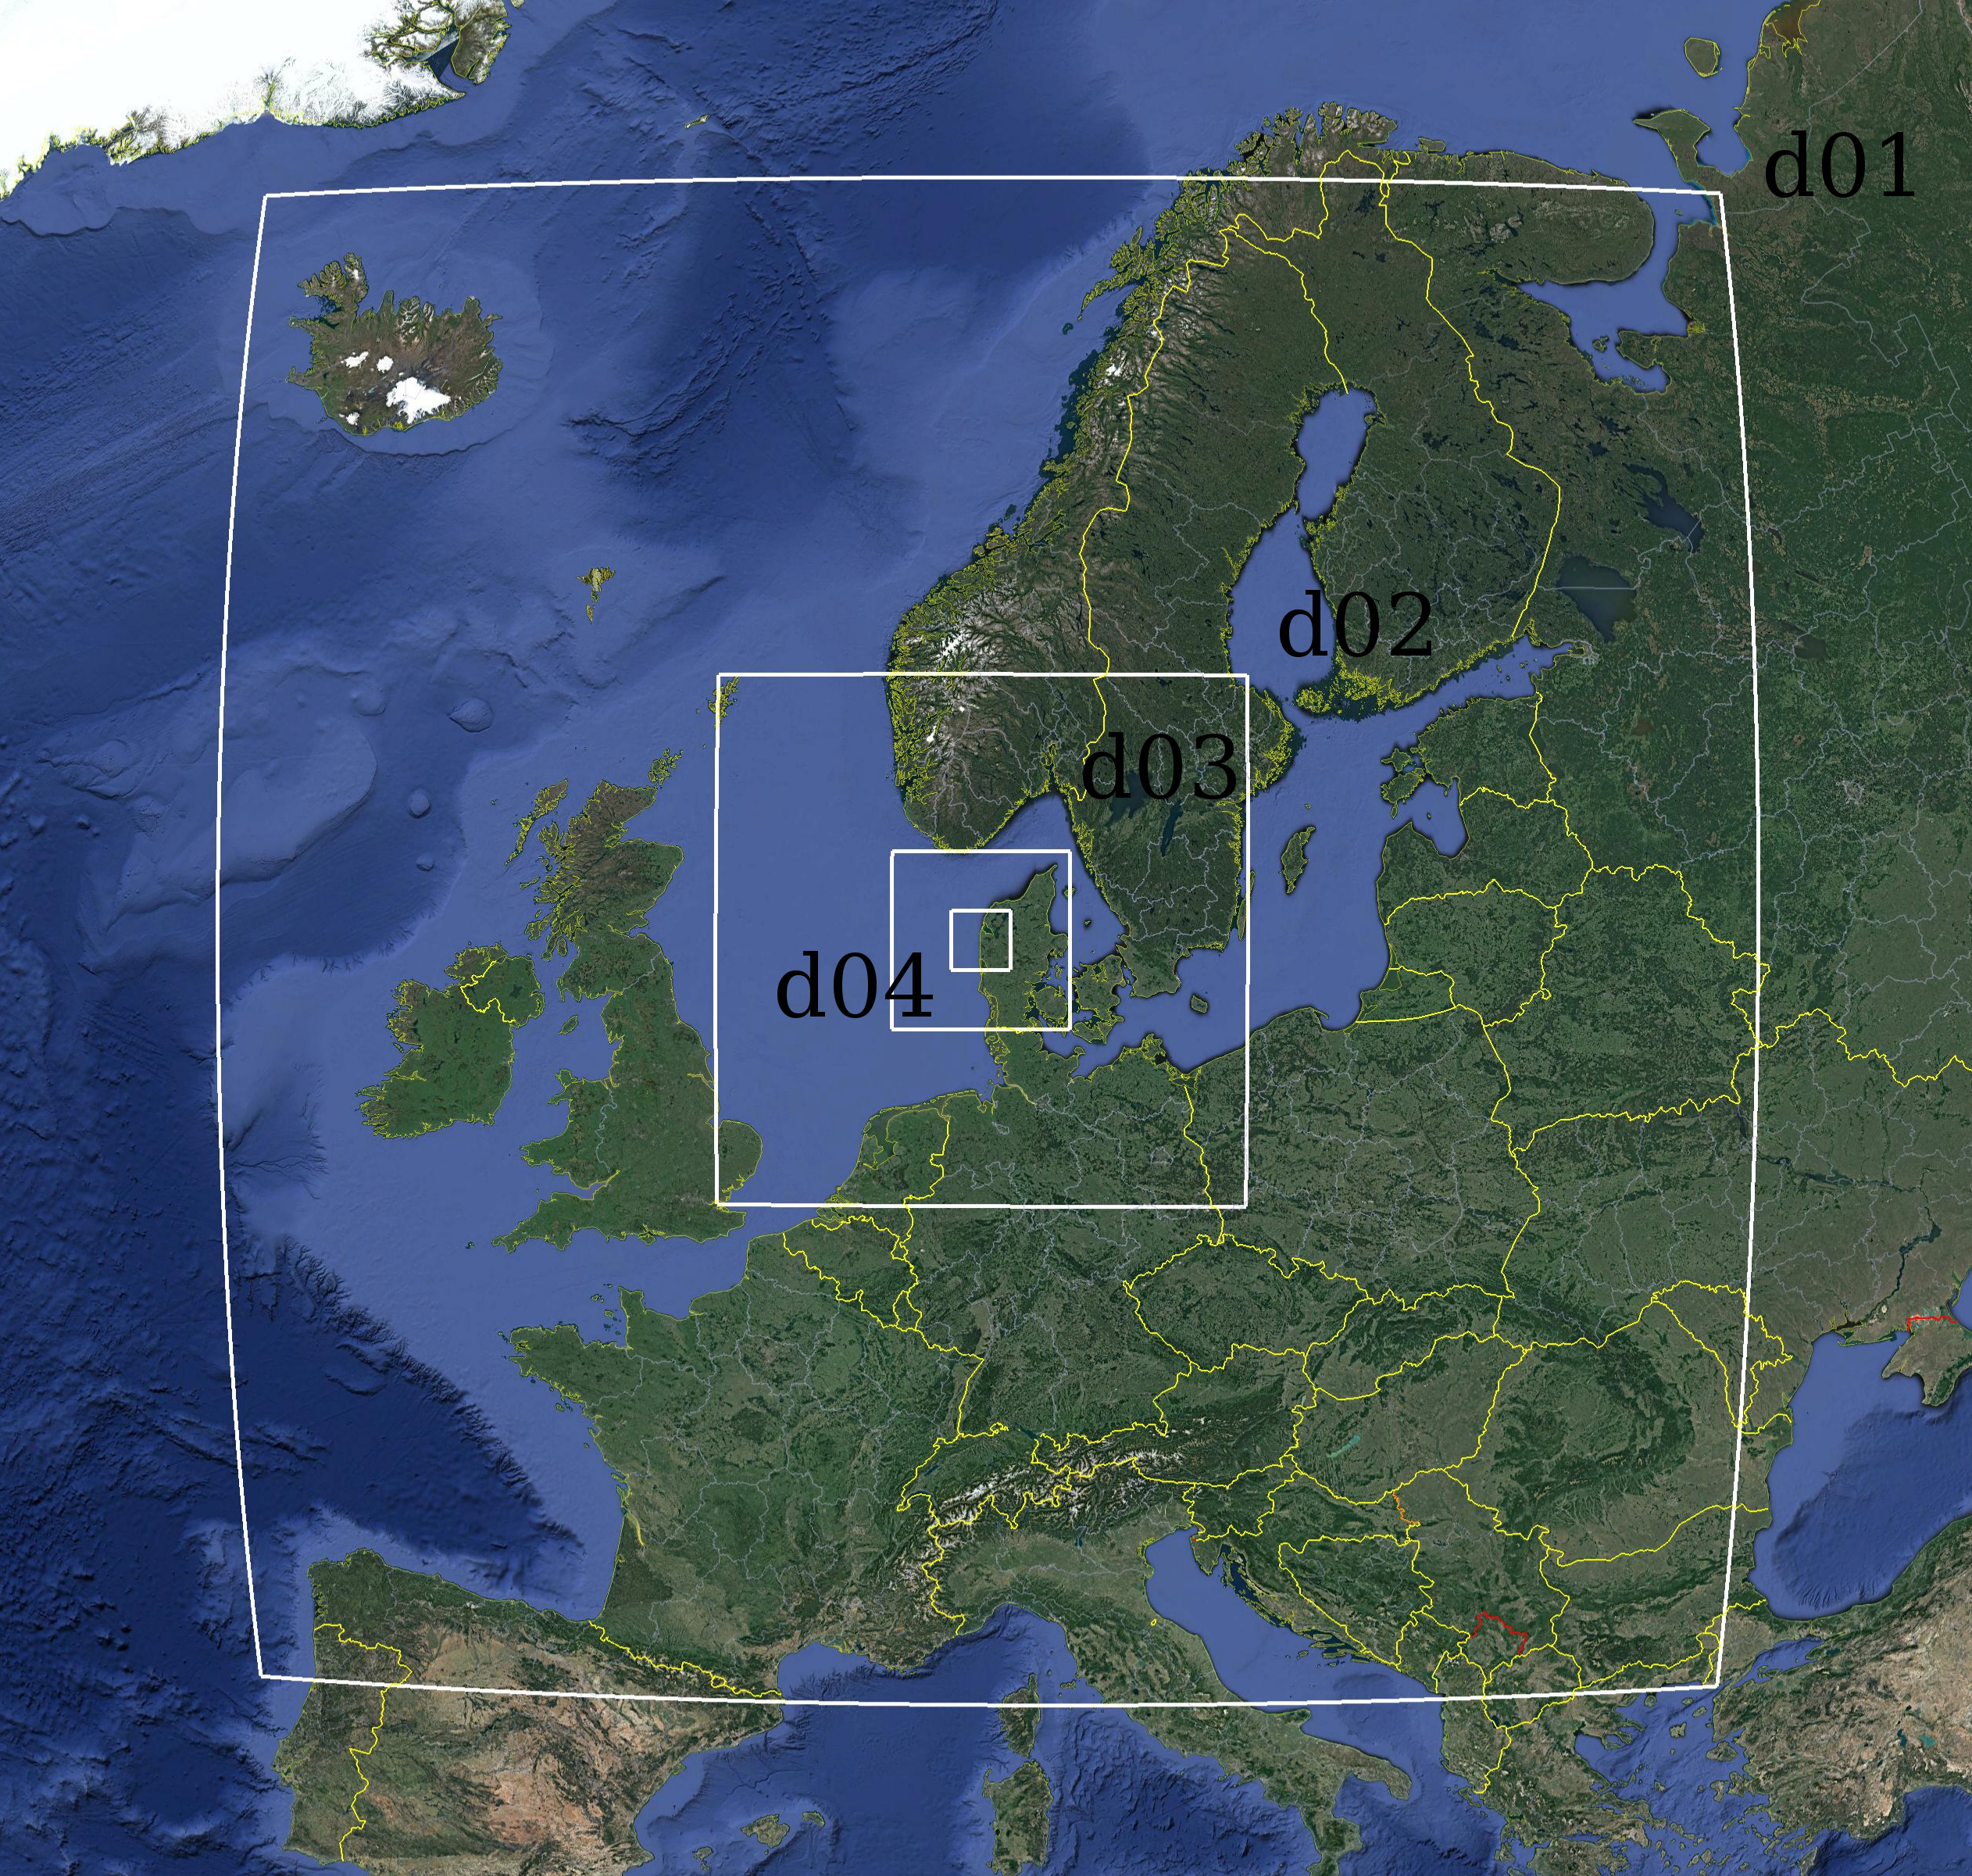
\includegraphics[width=0.6\linewidth,page=1,trim={5mm 3mm 3mm 3mm},clip,frame]{Imagenes/05/hov_dom1_edit.jpg}%
	
	\bigskip%
	
	\includegraphics[width=0.6\linewidth,page=1,trim={5mm 3mm 3mm 3mm},clip,frame]{Imagenes/05/hov_dom2_edit.jpg}%
	\caption{Distribución telescópica de los 7 mallas anidadas en el dominio numérico.}
	\label{fig:dom_telesco}
\end{figure}

\begin{figure}[H]
	\centering
	\includegraphics[width=0.25\linewidth,page=1,trim={2cm 6.5cm 1cm 3.5cm},clip]{Imagenes/05/hov_domain.pdf}%
	\includegraphics[width=0.25\linewidth,page=2,trim={2cm 6.5cm 1cm 3.5cm},clip]{Imagenes/05/hov_domain.pdf}%
	\includegraphics[width=0.25\linewidth,page=3,trim={2cm 6.5cm 1cm 3.5cm},clip]{Imagenes/05/hov_domain.pdf}%
	\includegraphics[width=0.25\linewidth,page=4,trim={2cm 6.5cm 1cm 3.5cm},clip]{Imagenes/05/hov_domain.pdf}%
	
	\bigskip
	\includegraphics[width=0.25\linewidth,page=5,trim={2cm 6.5cm 1cm 3.5cm},clip]{Imagenes/05/hov_domain.pdf}%
	\includegraphics[width=0.25\linewidth,page=6,trim={2cm 6.5cm 1cm 3.5cm},clip]{Imagenes/05/hov_domain.pdf}%
	\includegraphics[width=0.25\linewidth,page=7,trim={2cm 6.5cm 1cm 3.5cm},clip]{Imagenes/05/hov_domain.pdf}%
	\includegraphics[width=0.25\linewidth,page=8,trim={2cm 6.5cm 1cm 3.5cm},clip]{Imagenes/05/hov_domain.pdf}%
	
	\bigskip
	\includegraphics[width=0.25\linewidth,page=9,trim={2cm 6.5cm 1cm 3.5cm},clip]{Imagenes/05/hov_domain.pdf}%
	\includegraphics[width=0.25\linewidth,page=10,trim={2cm 6.5cm 1cm 3.5cm},clip]{Imagenes/05/hov_domain.pdf}%
	\includegraphics[width=0.25\linewidth,page=11,trim={2cm 6.5cm 1cm 3.5cm},clip]{Imagenes/05/hov_domain.pdf}%
	\includegraphics[width=0.25\linewidth,page=12,trim={2cm 6.5cm 1cm 3.5cm},clip]{Imagenes/05/hov_domain.pdf}%
	
	\bigskip
	\includegraphics[width=0.25\linewidth,page=1,trim={2cm 6.5cm 1cm 3.5cm},clip]{Imagenes/05/hov_control_point.pdf}%
	\includegraphics[width=0.25\linewidth,page=14,trim={2cm 6.5cm 1cm 3.5cm},clip]{Imagenes/05/hov_domain.pdf}%
	
	\caption{Orografía (MSNM) y uso de suelo (categoría USGS24) de alta definición para cada uno de las mallas anidadas (d01-d07). Para el dominio d07 se presenta la ubicación del punto de control (rojo) y la distribución de turbinas eólicas en la zona (negro).}
	\label{fig:dominios}
\end{figure}
\newpage
\begin{figure}[H]
	\centering
	\begin{minipage}{0.5\linewidth}
		\center(a)
	\end{minipage}%
	\begin{minipage}{0.5\linewidth}
		\center(b)
	\end{minipage}%
	
	\includegraphics[width=0.5\linewidth,trim={0cm 4cm -2cm 4cm},clip]{Imagenes/05/hov_mesh_y000001}%
	\includegraphics[width=0.5\linewidth,trim={0cm 4cm -2cm 4cm},clip]{Imagenes/05/hov_mesh_y000033}%
	
	\begin{minipage}{0.5\linewidth}
		\center(c)
	\end{minipage}%
	\begin{minipage}{0.5\linewidth}
		\center(d)
	\end{minipage}%
	
	\includegraphics[width=0.5\linewidth,trim={0cm 4cm -2cm 4cm},clip]{Imagenes/05/hov_mesh_y000066}%
	\includegraphics[width=0.5\linewidth,trim={0cm 4cm -2cm 4cm},clip]{Imagenes/05/hov_mesh_y000101}%
	
	\caption{Distribución de la malla vertical.}
	\label{fig:c1_mesh}
\end{figure}

\subsection{Aspectos generales del proceso de asimilación de datos}
A modo de implementar una mejora para la simulación multiescala a alta resolución que se está realizando, es que se plantea la utilización de un método de asimilación de datos para poder anclar ciertos valores conocidos dentro de la simulación y así obtener resultados mas acordes a la realidad.

La base teórica de la asimilación de datos en WRF ya se mencionó en informes anteriores. A continuación se presentan la información relevante para la correcta ejecución del sistema de asimilación y su replicabilidad.

\begin{table}[h!]
	\caption{Características del proceso de DA.}\label{tab:c2DA}
	\centering\footnotesize
	\begin{tabular}{lcc}
		\toprule
		Parámetro & Selección \\
		\midrule
		Hora Inicio	DA 	 & 06:00:00   \\
		Hora Término DA	 		 & 12:00:00  \\
		Intervalo de DA	&	10 mins. \\
		Puntos a Anidar	 	 & 5   \\
		Variables	& $u,v$   \\
		Lat. Mástil	& 56.440582   \\
		Lon. Mástil	& 8.150896   \\
		Alturas 	& 10m, 40m, 60m, 80m, 100m \\
		\bottomrule
	\end{tabular}
\end{table}

Los valores a asimilar son los valores tomados experimentalmente en el mástil meteorológico de Høvsøre y que se pueden ver en la Figura \ref{fig:ts_u}.

\newpage
\section{Caso de Estudio: Terreno Complejo Bolund}
\subsection{Aspectos generales de las simulaciones}
Tomando en cuenta que la campaña de medición para el caso Bolund se llevó a cabo durante los meses de Enero y Febrero del 2008, fue necesario hallar un día en donde hubiera una estratificación atmosférica lo mas neutra posible, con el modo de tener resultados comparables con aquellos obtenidos en la literatura y simulados de manera ideal.

Convenientemente, en el informe técnico que detalla la campaña de medición, los autores presentan un gráfico para la longitud de Monin-Obukhov que permite identificar que los días 3-4 de Enero presentan una estratificación muy cercana a la neutra y por lo tanto se decide simular para esas horas.
\begin{table}[h!]
	\caption{Dominio numerico espacial y temporal para simulación del caso Høvsøre.}\label{tab:c3exp}
	\centering\footnotesize
	\begin{tabular}{lcc}
		\toprule
		Parámetro & Selección \\
		\midrule
		Fecha	 	 & 04-01-2008   \\
		Hora Inicio	 	 & 06:00 UTM\\
		Hora Término	 		 & 20:00 UTM\\
		Puntos Malla Vert.	 	 & 50   \\
		$P_{top}$ 	& 10000 kPa\\
		\# Dominios	& 8   \\
		Lat. Centro	& 55.70360   \\
		Lon. Centro	& 12.09840   \\
		\bottomrule
	\end{tabular}
\end{table}

\begin{table}[H]
	\caption{Valores característicos de cada dominio.}\label{tab:c3val_carac}
	\centering\footnotesize
	\begin{tabular}{lllllllll}
		\toprule
		Dominio 				& d01	&	d02	&	d03	&	d04	&	d05	&	d06 &	d07&	d08 \\
		\midrule
		$N_x$		& 106 & 106 & 106 &106&106&106&106&106  \\
		$N_y$	 		& 106 & 106 & 106 &106&106&106&106&91  \\
		$\Delta x,\Delta y$	[m]	 		& 10000 & 3333.3 & 1111.1 &222.22&74.074&24.691&8.23045&2.74348  \\
		$\Delta t$	[s]	 		& 40 & 13.3333 & 4.4444 &0.8889&0.2963&0.0988&0.0329&0.0110  \\
		Orografía		 	& GMTED2010 & GMTED2010 & GMTED2010 &ASTER&ASTER&ASTER&ASTER&Bolund  \\
		Uso de Suelo					& USGS & USGS & USGS &CLC12&CLC12&CLC12&CLC12&Bolund \\
		\bottomrule
	\end{tabular}
\end{table}

\begin{table}[H]
	\caption{Parametrizaciones físicas utilizadas en el modelo.}\label{tab:c3param_fis}
	\centering\footnotesize
	\begin{tabular}{llllllll}
		\toprule
		Dominio 				& d01	&	d02	&	d03	&	d04	&	d05	&	d06 &	d07 \\
		\midrule
		Micro-físicas		 	& WSM5 & WSM5 & WSM5 &WSM5&WSM5&WSM5&WSM5  \\
		Cúmulos			 		& Grell & -- & -- & -- & -- & -- & -- \\ 
		Capa Superficial	 	& MM5 & MM5 & MM5 & MM5 & MM5 & MM5 & MM5 \\
		PBL				 		& YSU & YSU & YSU & -- & -- & -- & -- \\
		Modelo LES				 		& -- & -- & -- & 1.5TKE & 1.5TKE & 1.5TKE & 1.5TKE \\
		Modelo de Suelo 		& Difus. & Difus. & Difus. & Difus. & Difus. & Difus. & Difus. \\
		Rad. Onda Larga	& RRTM &RRTM&RRTM&RRTM&RRTM&RRTM&RRTM \\
		Rad. Onda Corta	& Dudhia &Dudhia&Dudhia&Dudhia&Dudhia&Dudhia&Dudhia \\
		\bottomrule
	\end{tabular}
\end{table}

\begin{figure}[H]
	\centering
	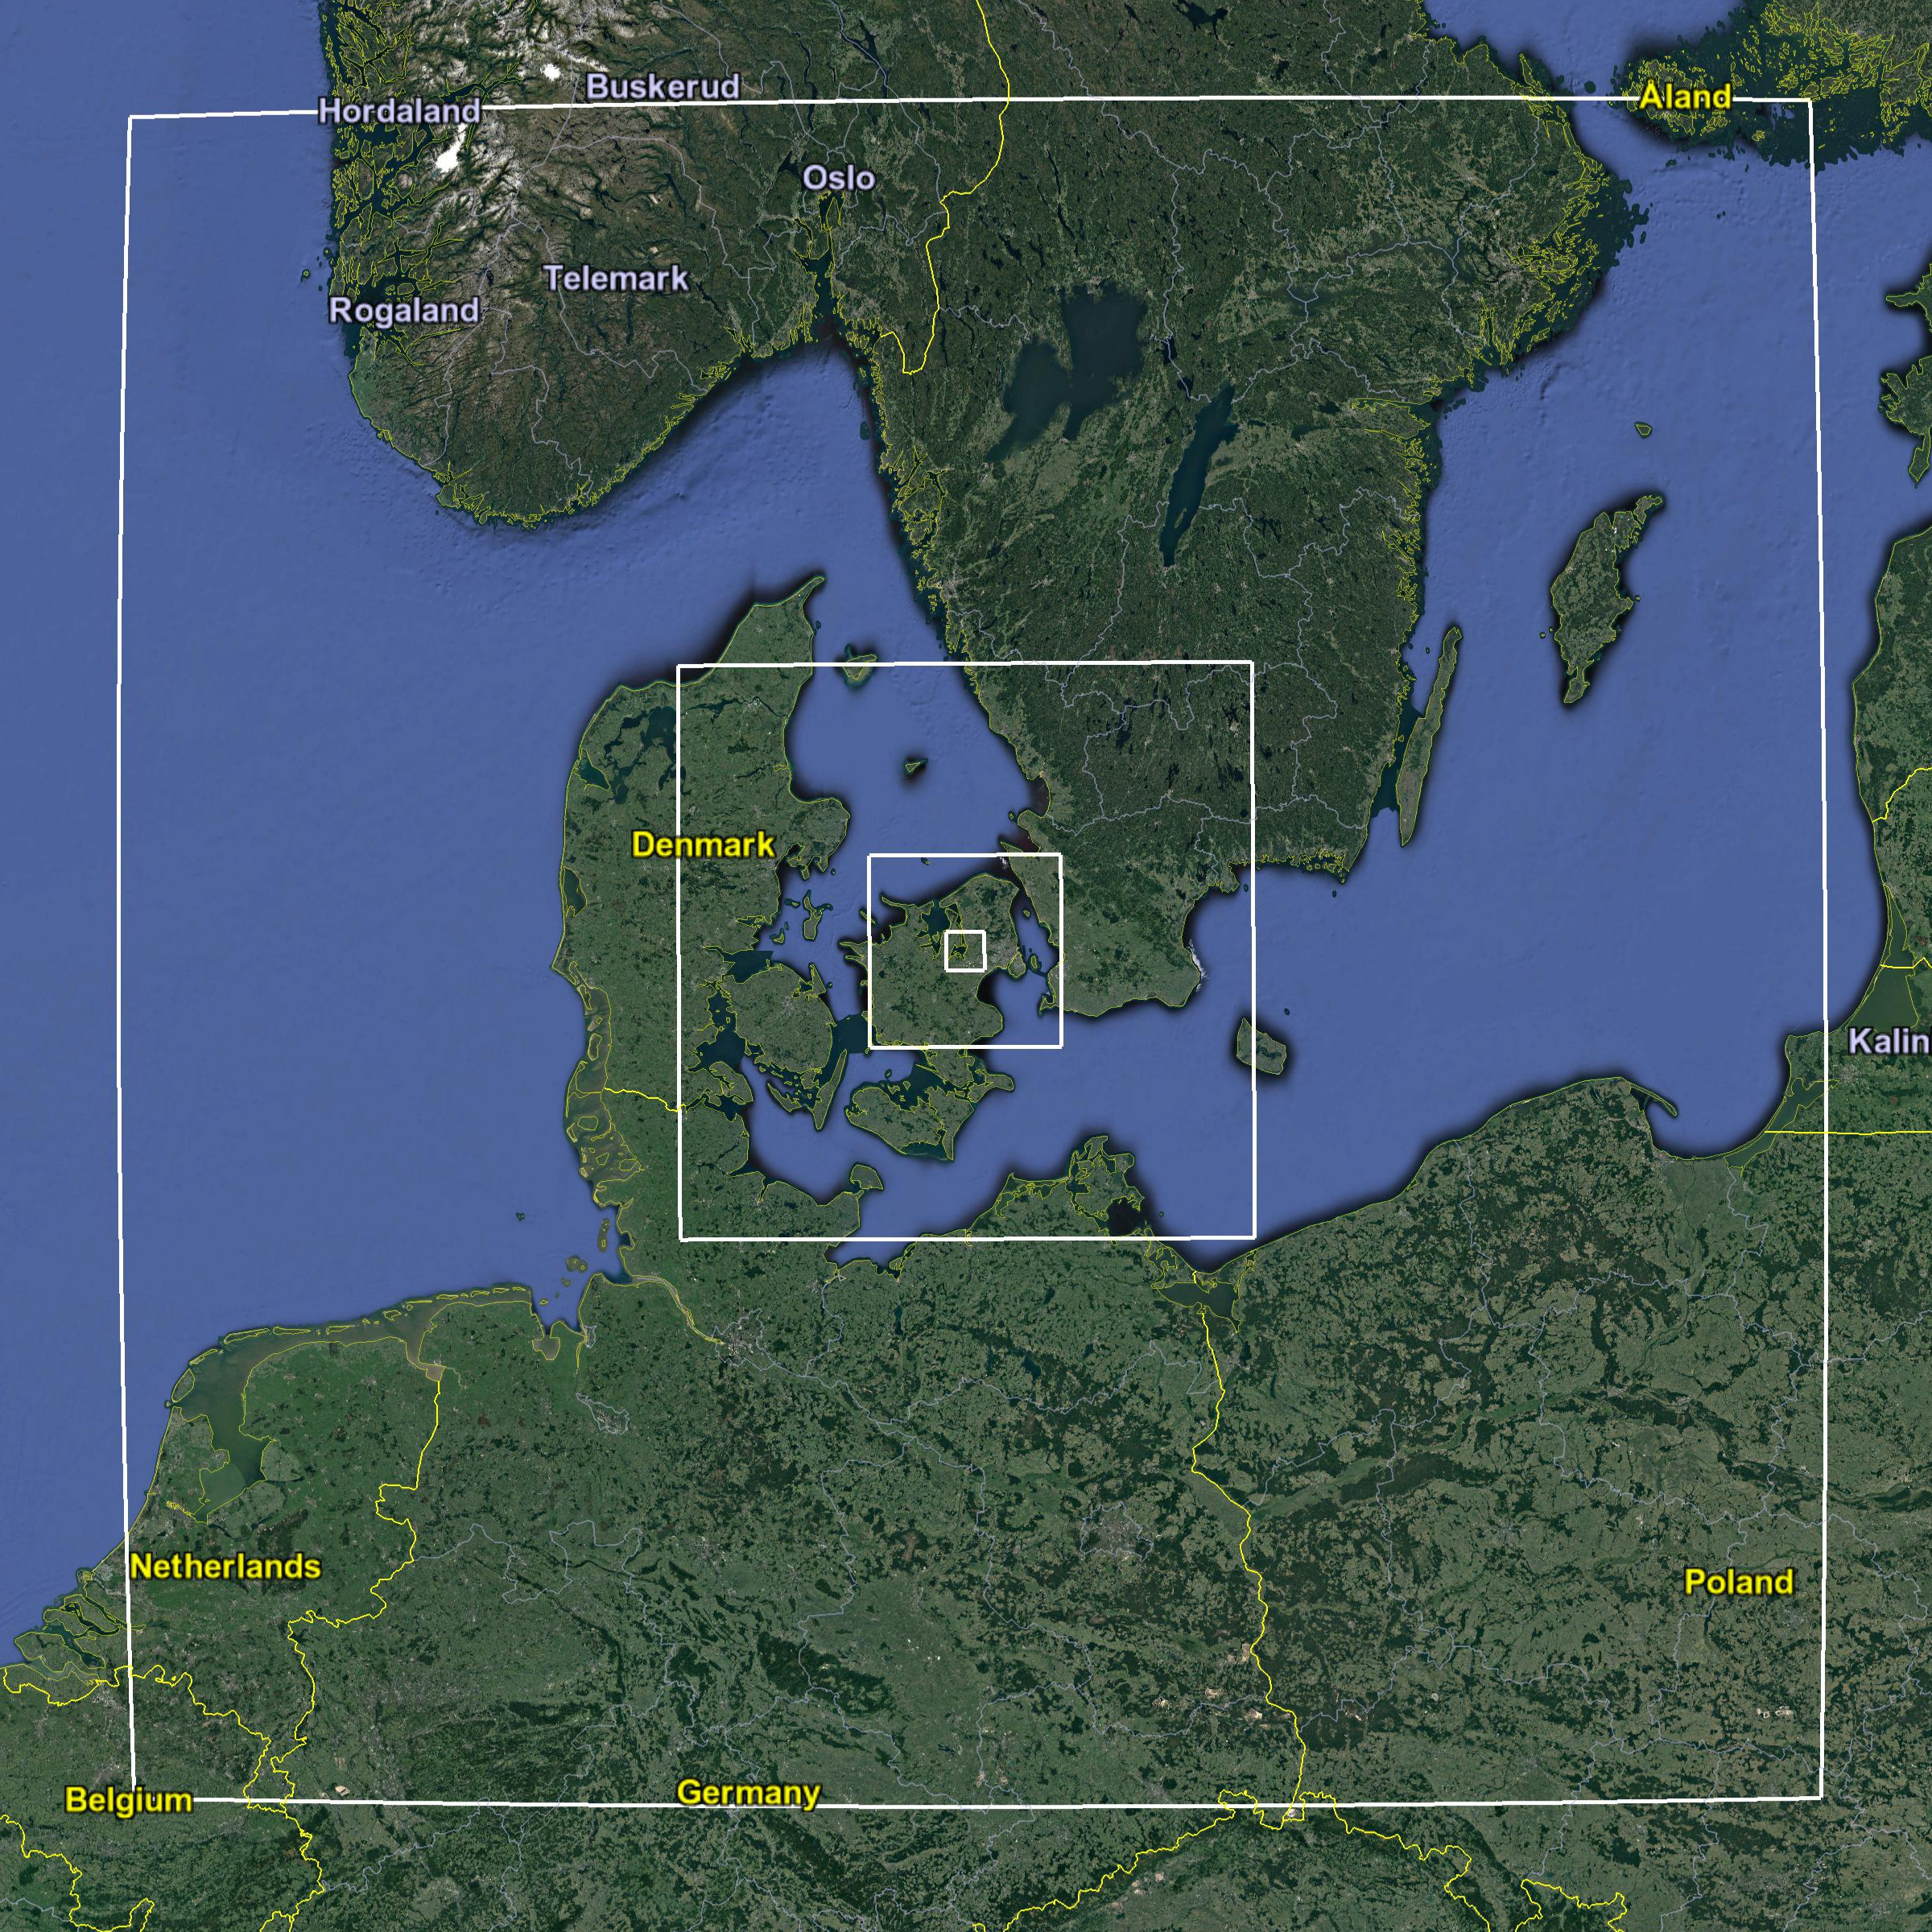
\includegraphics[width=0.48\linewidth,page=1,trim={5mm 3mm 3mm 3mm},clip,frame]{Imagenes/05/bol_d1-2-3-4edit.jpg}
	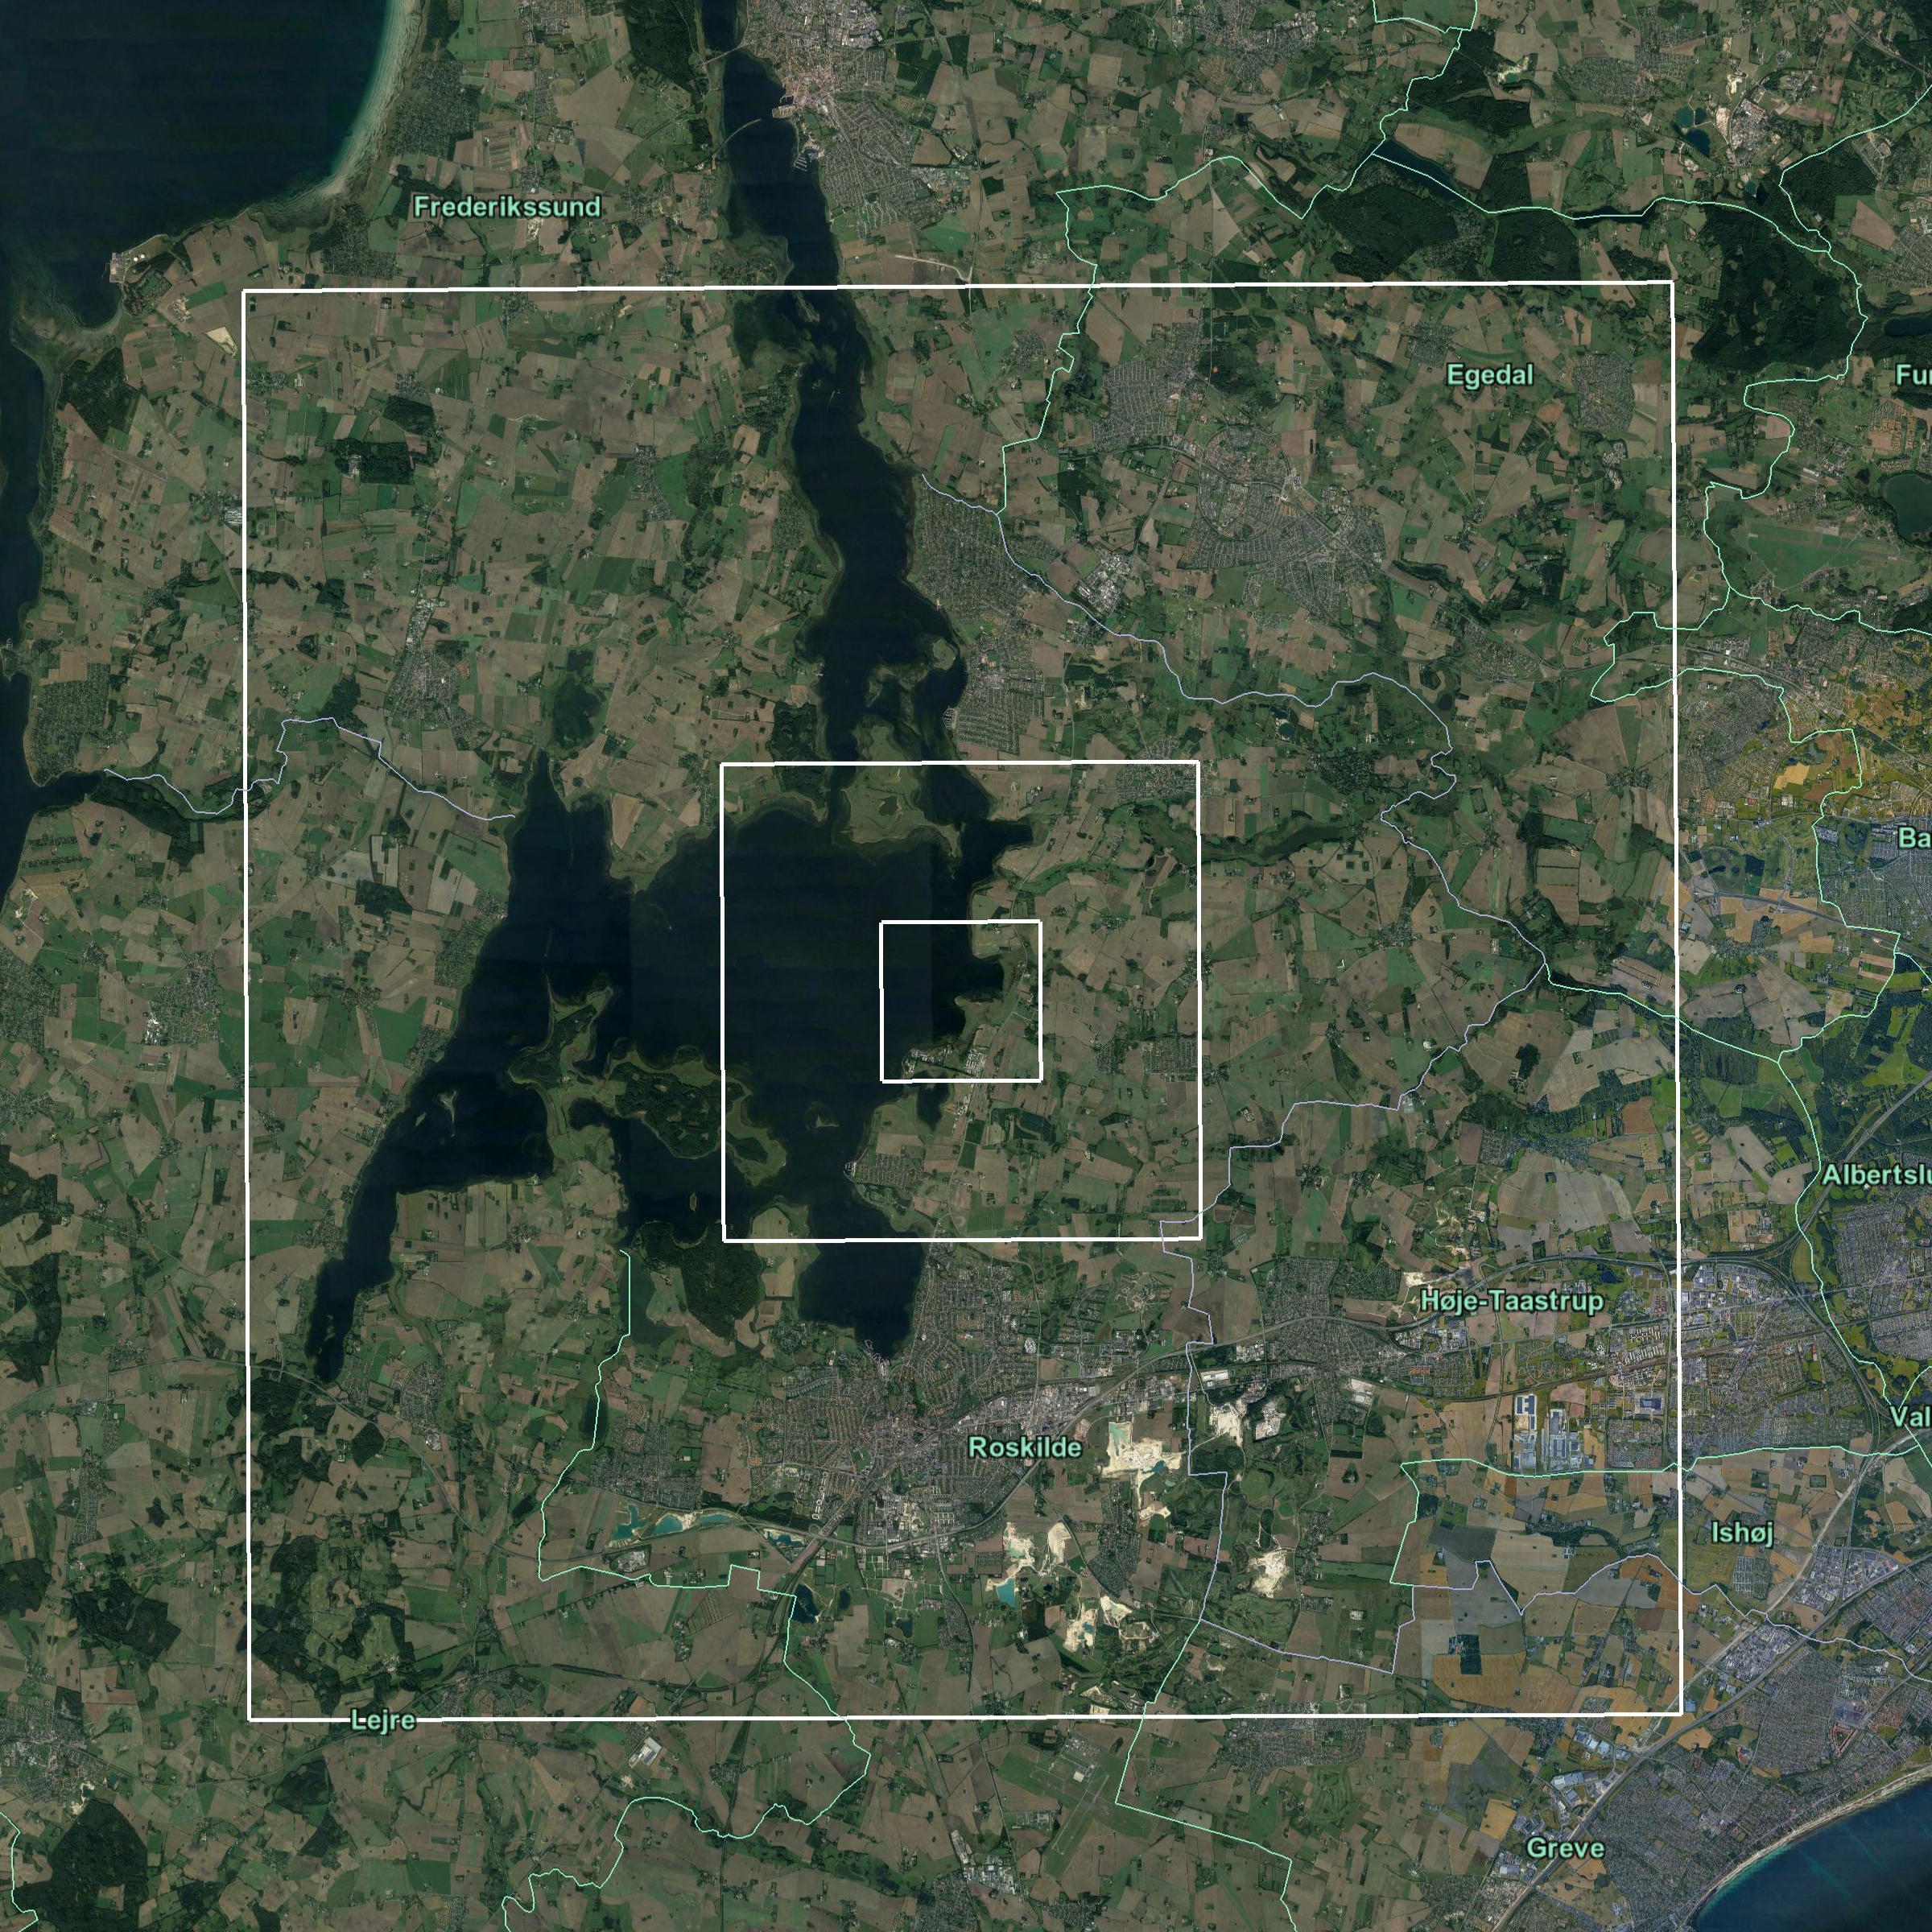
\includegraphics[width=0.48\linewidth,page=1,trim={5mm 3mm 3mm 3mm},clip,frame]{Imagenes/05/bol_d4-5-6edit.jpg}
	
	\bigskip
	\includegraphics[width=0.6\linewidth,page=1,trim={5mm 3mm 3mm 3mm},clip,frame]{Imagenes/05/bol_d6-7-8edit.jpg}%
	
	\caption{Distribución telescópica de los 8 mallas anidadas en el dominio numérico.}
	\label{fig:c3dom_telesco}
\end{figure}

\begin{figure}[H]
	\centering
	\includegraphics[width=0.25\linewidth,page=1,trim={2cm 6.5cm 1cm 3.5cm},clip]{Imagenes/05/bol_domain.pdf}%
	\includegraphics[width=0.25\linewidth,page=2,trim={2cm 6.5cm 1cm 3.5cm},clip]{Imagenes/05/bol_domain.pdf}%
	\includegraphics[width=0.25\linewidth,page=3,trim={2cm 6.5cm 1cm 3.5cm},clip]{Imagenes/05/bol_domain.pdf}%
	\includegraphics[width=0.25\linewidth,page=4,trim={2cm 6.5cm 1cm 3.5cm},clip]{Imagenes/05/bol_domain.pdf}%
	
	\bigskip
	\includegraphics[width=0.25\linewidth,page=5,trim={2cm 6.5cm 1cm 3.5cm},clip]{Imagenes/05/bol_domain.pdf}%
	\includegraphics[width=0.25\linewidth,page=6,trim={2cm 6.5cm 1cm 3.5cm},clip]{Imagenes/05/bol_domain.pdf}%
	\includegraphics[width=0.25\linewidth,page=7,trim={2cm 6.5cm 1cm 3.5cm},clip]{Imagenes/05/bol_domain.pdf}%
	\includegraphics[width=0.25\linewidth,page=8,trim={2cm 6.5cm 1cm 3.5cm},clip]{Imagenes/05/bol_domain.pdf}%
	
	\bigskip
	\includegraphics[width=0.25\linewidth,page=9,trim={2cm 6.5cm 1cm 3.5cm},clip]{Imagenes/05/bol_domain.pdf}%
	\includegraphics[width=0.25\linewidth,page=10,trim={2cm 6.5cm 1cm 3.5cm},clip]{Imagenes/05/bol_domain.pdf}%
	\includegraphics[width=0.25\linewidth,page=11,trim={2cm 6.5cm 1cm 3.5cm},clip]{Imagenes/05/bol_domain.pdf}%
	\includegraphics[width=0.25\linewidth,page=12,trim={2cm 6.5cm 1cm 3.5cm},clip]{Imagenes/05/bol_domain.pdf}%
	
	\bigskip
	\includegraphics[width=0.25\linewidth,page=13,trim={2cm 6.5cm 1cm 3.5cm},clip]{Imagenes/05/bol_domain.pdf}%
	\includegraphics[width=0.25\linewidth,page=14,trim={2cm 6.5cm 1cm 3.5cm},clip]{Imagenes/05/bol_domain.pdf}%
	
	\bigskip
	\includegraphics[width=0.25\linewidth,page=15,trim={0cm 6.5cm 1cm 3.5cm},clip]{Imagenes/05/bol_domain.pdf}%
	\includegraphics[width=0.25\linewidth,page=16,trim={0cm 6.5cm 1cm 3.5cm},clip]{Imagenes/05/bol_domain.pdf}%
	
	\caption{Orografía (MSNM) y uso de suelo (categoría USGS24) de alta definición para cada uno de las mallas anidadas (d01-d08).}
	\label{fig:c3dominios}
\end{figure}

\begin{figure}[H]
	\centering
	\includegraphics[width=0.9\linewidth,page=1,trim={0cm 6cm -1cm 4cm},clip]{Imagenes/05/bol_control_point.pdf}%
	\caption{Ubicación espacial de los puntos de control en el dominio. En cada punto de control se ubican anemómetros que miden a las alturas de 2m, 5m, y 9m.}
	\label{fig:c3control_points}
\end{figure}

\begin{figure}[H]
	\centering
	\begin{minipage}{0.5\linewidth}
		\center(a)
	\end{minipage}%
	\begin{minipage}{0.5\linewidth}
		\center(b)
	\end{minipage}%
	
	\includegraphics[width=0.5\linewidth,trim={3cm 0cm 0cm 0cm},clip]{Imagenes/05/bol_mesh_y000001}%
	\includegraphics[width=0.5\linewidth,trim={3cm 0cm 0cm 0cm},clip]{Imagenes/05/bol_mesh_y000022}%
	
	\begin{minipage}{0.5\linewidth}
		\center(c)
	\end{minipage}%
	\begin{minipage}{0.5\linewidth}
		\center(d)
	\end{minipage}%
	
	\includegraphics[width=0.5\linewidth,trim={3cm 0cm 0cm 0cm},clip]{Imagenes/05/bol_mesh_y000053}%
	\includegraphics[width=0.5\linewidth,trim={3cm 0cm 0cm 0cm},clip]{Imagenes/05/bol_mesh_y000090}%
	
	\caption{Distribución de la malla vertical.}
	\label{fig:c3_mesh}
\end{figure}

\subsection{Aspectos generales del proceso de asimilación de datos}

\begin{table}[h!]
	\caption{Características del proceso de DA.}\label{tab:c2DA}
	\centering\footnotesize
	\begin{tabular}{lcc}
		\toprule
		Parámetro & Selección \\
		\midrule
		Hora Inicio	DA 	 & 06:00:00   \\
		Hora Término DA	 		 & 12:00:00  \\
		Intervalo de DA	&	10 mins. \\
		Puntos a Anidar	 	 & ??   \\
		Variables	& $u,v$   \\
		Lat. Mástil	& ??   \\
		Lon. Mástil	& ??   \\
		Alturas 	& 2m, 5m, 9m \\
		\bottomrule
	\end{tabular}
\end{table}
